\subsection{Finding Resonance} \label{B1}

To begin, the NMR spectrometer settings were adjusted explore how they impact an FID signal for the doped water sample. Adjusting the repetition time had no measurable impact on the signal, indicating that water spin-lattice relaxation (regrowth) time is less than (or equal to) the lowest repetition time setting of 0.3 seconds. The receiver gain was not adjusted as increasing it reduced the signal-to-noise ratio of the spectrometer. The receiver phase and the 90 degree pulse dial were adjusted to maximize the signal. Adjusting the 90 degree pulse dial adjusts the amount of time that the sample experiences the applied magnetic field, $B_1$. In our system, the magnetization vector, $\vec{M}$, begins pointing in the direction of $B_0$, which is defined as the $z$-direction. The $B_1$ field is applied in such a way that it rotates the $\vec{M}$ vector into the desired orientation. A 90 degree pulse, as shown in Figure \ref{fig:B1:pulses}, occurs when the $B_1$ field has been applied until $\vec{M}$ points along the $xy$-axis. As our detection system is designed to measure the magnetization along the $x$-axis, the signal is maximized for this type of pulse. \\

Similarly, for a 180 degree pulse $M$ is pointing in the negative $z$-direction and the signal is reduced to approximately zero. For a 270 degree pulse, the signal is minimized (negative peak) as it is pointing along the negative $x$ direction.\\

%The signal decay is caused by the individual spins are spinning at a different frequencies. The different frequencies are caused by inhomogeneities in $B_0$ and the intermolecular forces. If you imagine the spin vectors in a reference frame that is rotating at the Larmour frequency, when $B_1$ field is applied then, for a 90 degree pulse for example, the individual spins all align along the x axis. After the $B_1$ is no longer applied, the vectors start dephasing in the xy plane. The vectors will go out of phase if the spin has a frequency different than the Larmour frequency. Over time, the phasors will completely dephase and add to 0. 

\begin{figure}[H]
    \centering
    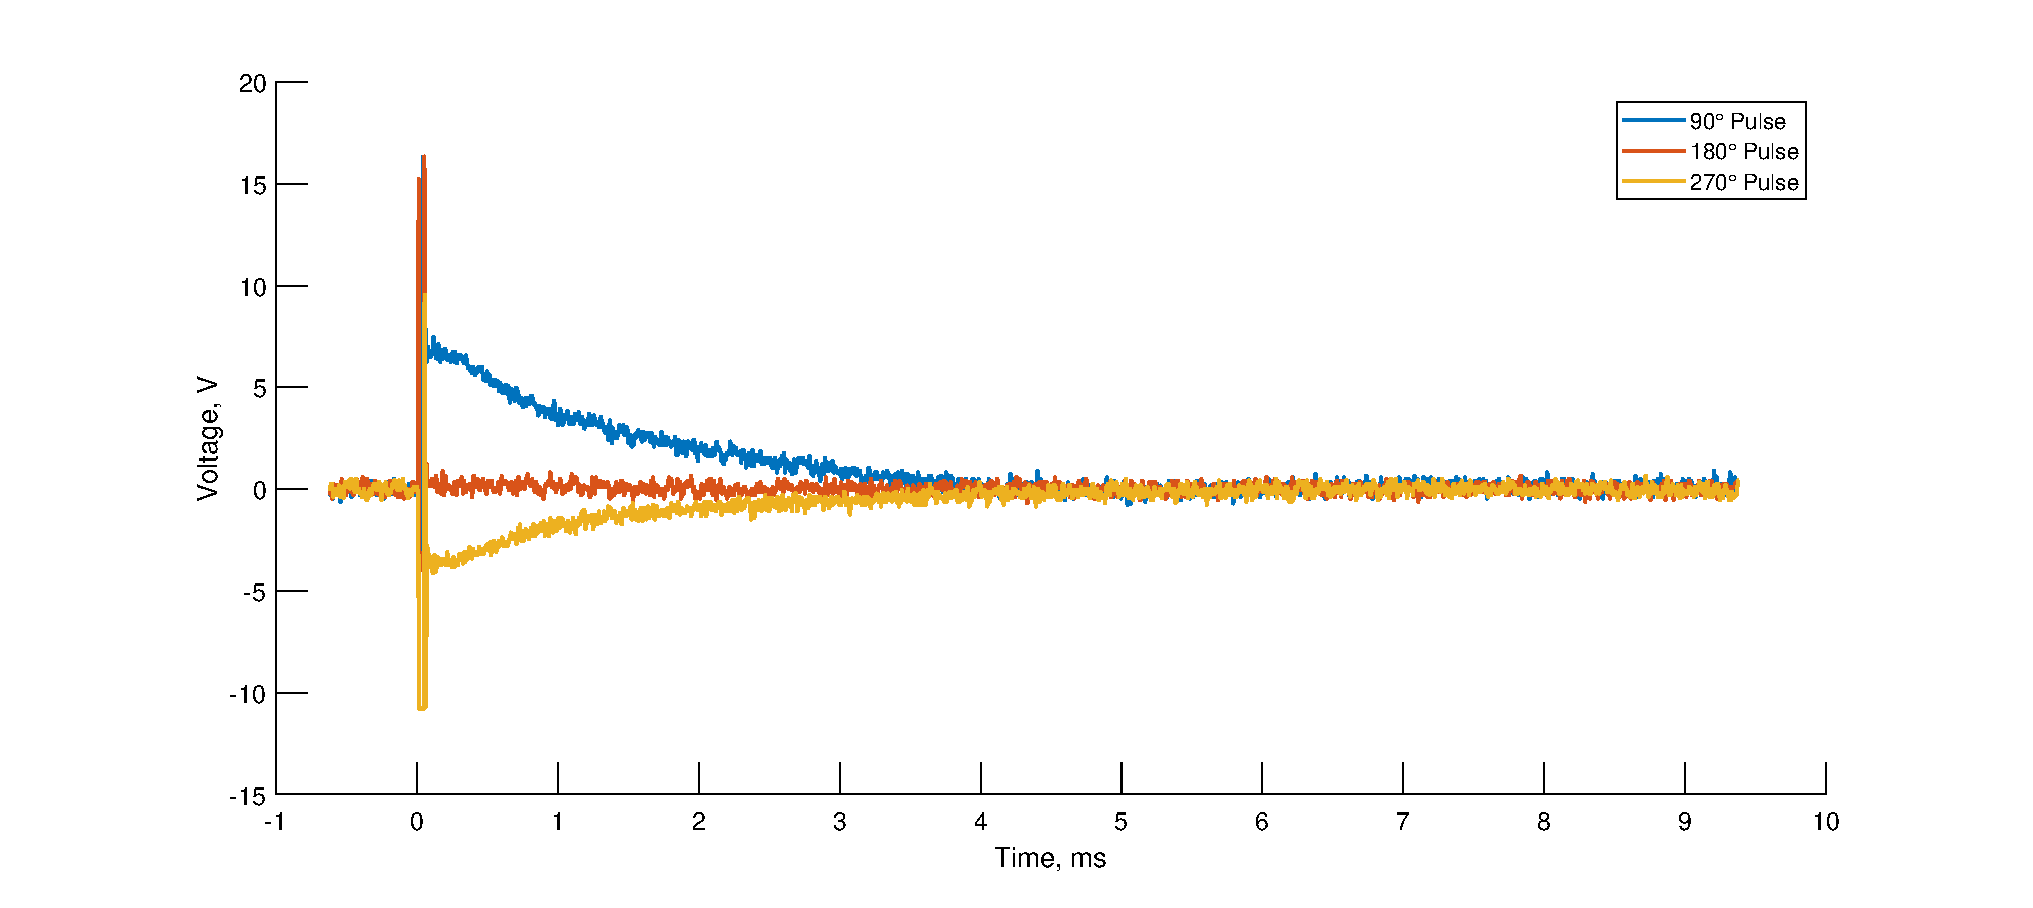
\includegraphics[width=\textwidth]{figures/B1/B1_1.eps}
    \caption{FID of doped water for a 90, 180 and 270 degree pulses.}
    \label{fig:B1:pulses}
\end{figure}


%Figure 5.2 was theoretically supposed to show a 180 degree pulse but the depicted pulse is greater than 180 because there is a negative amplitude, suggesting that there is a negative x component to the signal.

\subsection{Finding \texorpdfstring{$T_{2}^*$}{T2*} for Water, Ethanol and Rubber} \label{B2}

Similar to Section \ref{B1}, the FID of three samples (doped water, ethanol, and rubber) were measured for 90 degree pulses only. The repetition rate, detector phase, and pulse value were set to maximize the signal for each sample.\\

The magnetization as a function of time for the FID experiment is given by the expression,
\begin{align*}
    M_y(t) &= M_0 e^{-t/T_2^*} \numberthis\label{eqn:B2:eqn1} \\
    \intertext{Taking the natural logarithm of both sides of this expression,}
    \ln(M_y(t)) &= -t/T_2^* + \ln(M_0) \numberthis \label{eqn:B2:logfit}
\end{align*}

The first method to calculate $T_2^*$ is an approximation method. From Equation \ref{eqn:B2:eqn1}, when $t=T_2^*$ the magnetization is $M_y=M_0/e$; thus by calculating the time where the magnetization has decayed to this value is an approximate value of $T_2^*$. From the FID of each sample, the peak magnetization $M_0$ is measured and the intersection of the decay slope with $M_0/e$ is calculated. This is demonstrated in Figure \ref{fig:B2:T2*_approx} for doped water, and the estimated values of $T_2^*$ are summarized in Table \ref{tab:B2:T2*_values} (see Figure \ref{fig:A_B2_estimate} in Appendix for $T_2^*$ estimation plots for ethanol and rubber). The uncertainty values in our estimated time constant are taken as the uncertainty in determining $M_0$. This method is highly inaccurate, and is used only as an initial estimation.
\begin{figure}[H]
\centering
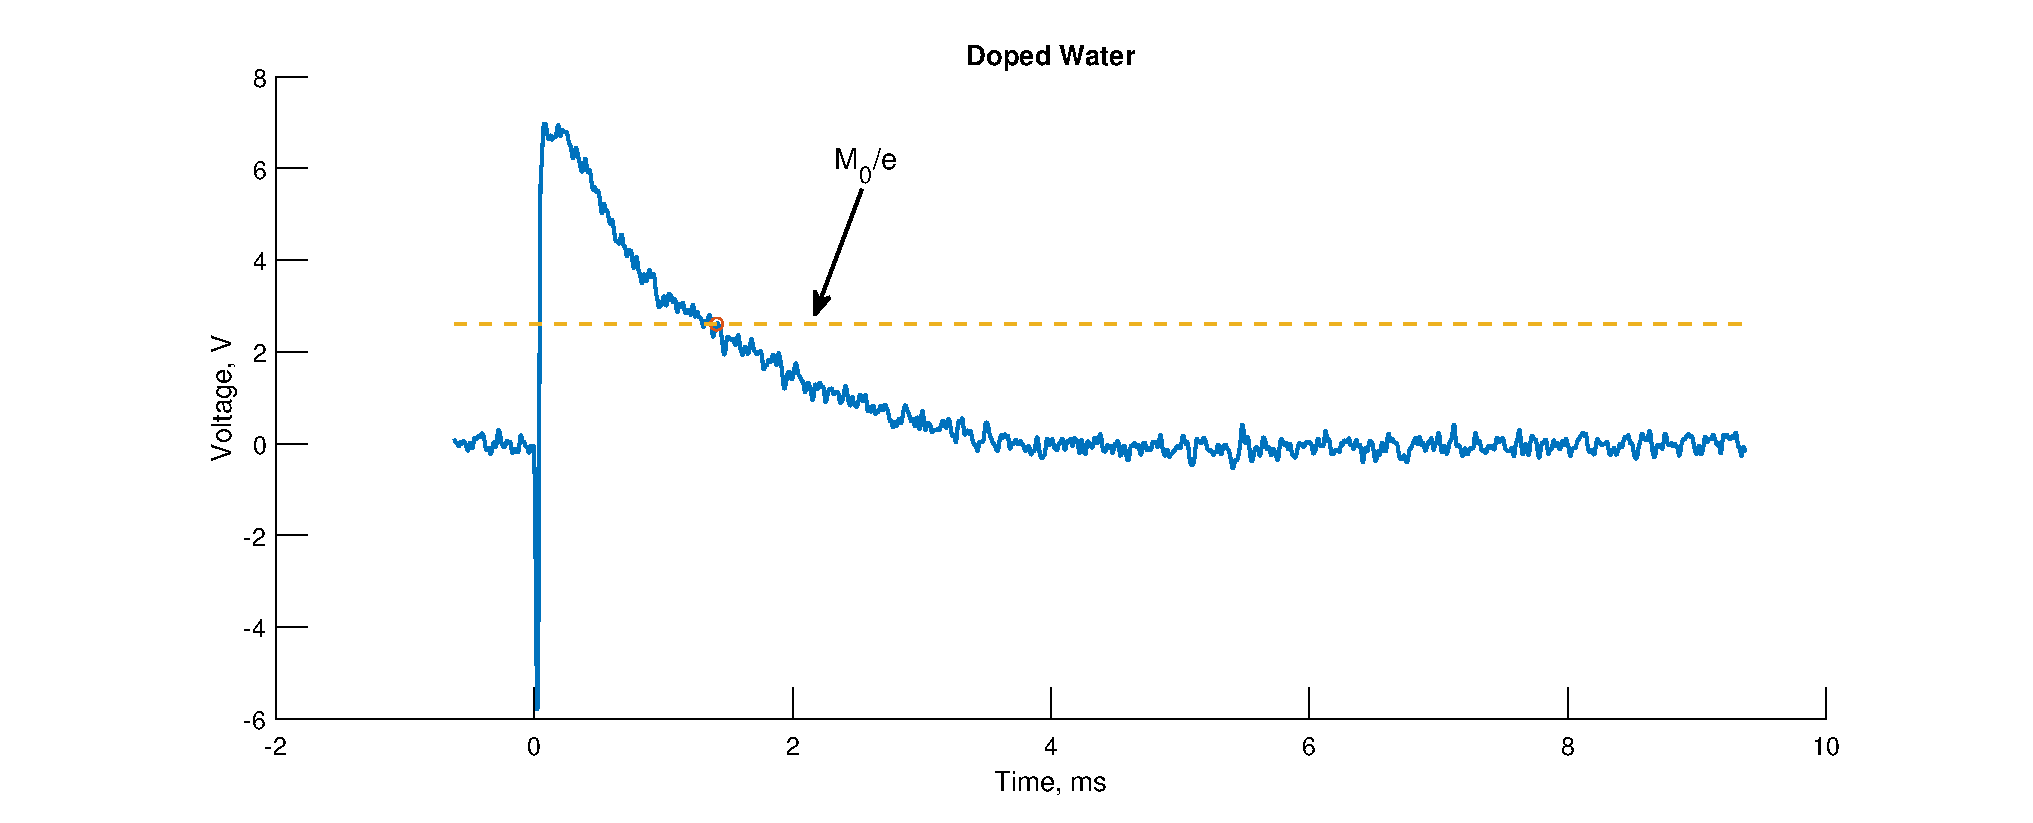
\includegraphics[width=\textwidth]{figures/B2/B2_2.eps}
\caption{Estimation of $T_2^*$ for doped water using the time value where $M_y\approx M_0/e$. Values for other samples are tabulated in Table \ref{tab:B2:T2*_values}.}
\label{fig:B2:T2*_approx}
\end{figure}

A more accurate method of calculating the time constant $T_2^*$ is to use a linear fit with the form of Equation \ref{eqn:B2:logfit}. Prior to fitting, each data set was zero shifted; and no filtering was performed for these data sets. The natural logarithm of the magnetization was fit with a linear slope using the method of least squares. Only the portion of the data set which contained a strong signal was used in the fitting process, as the signal to noise ratio with the rest of the data set is too low to generate an accurate value of $T_2^*$. The uncertainty in these measurements are regarded as the 95\% confidence interval of the fitting algorithm. Figure \ref{fig:B2:T2*_samples} demonstrates the fits for each sample (note that this plot demonstrates the fit data converted back to exponential form, to demonstrate the accuracy of the fit to the raw data).\\

\begin{figure}[H]
\centering
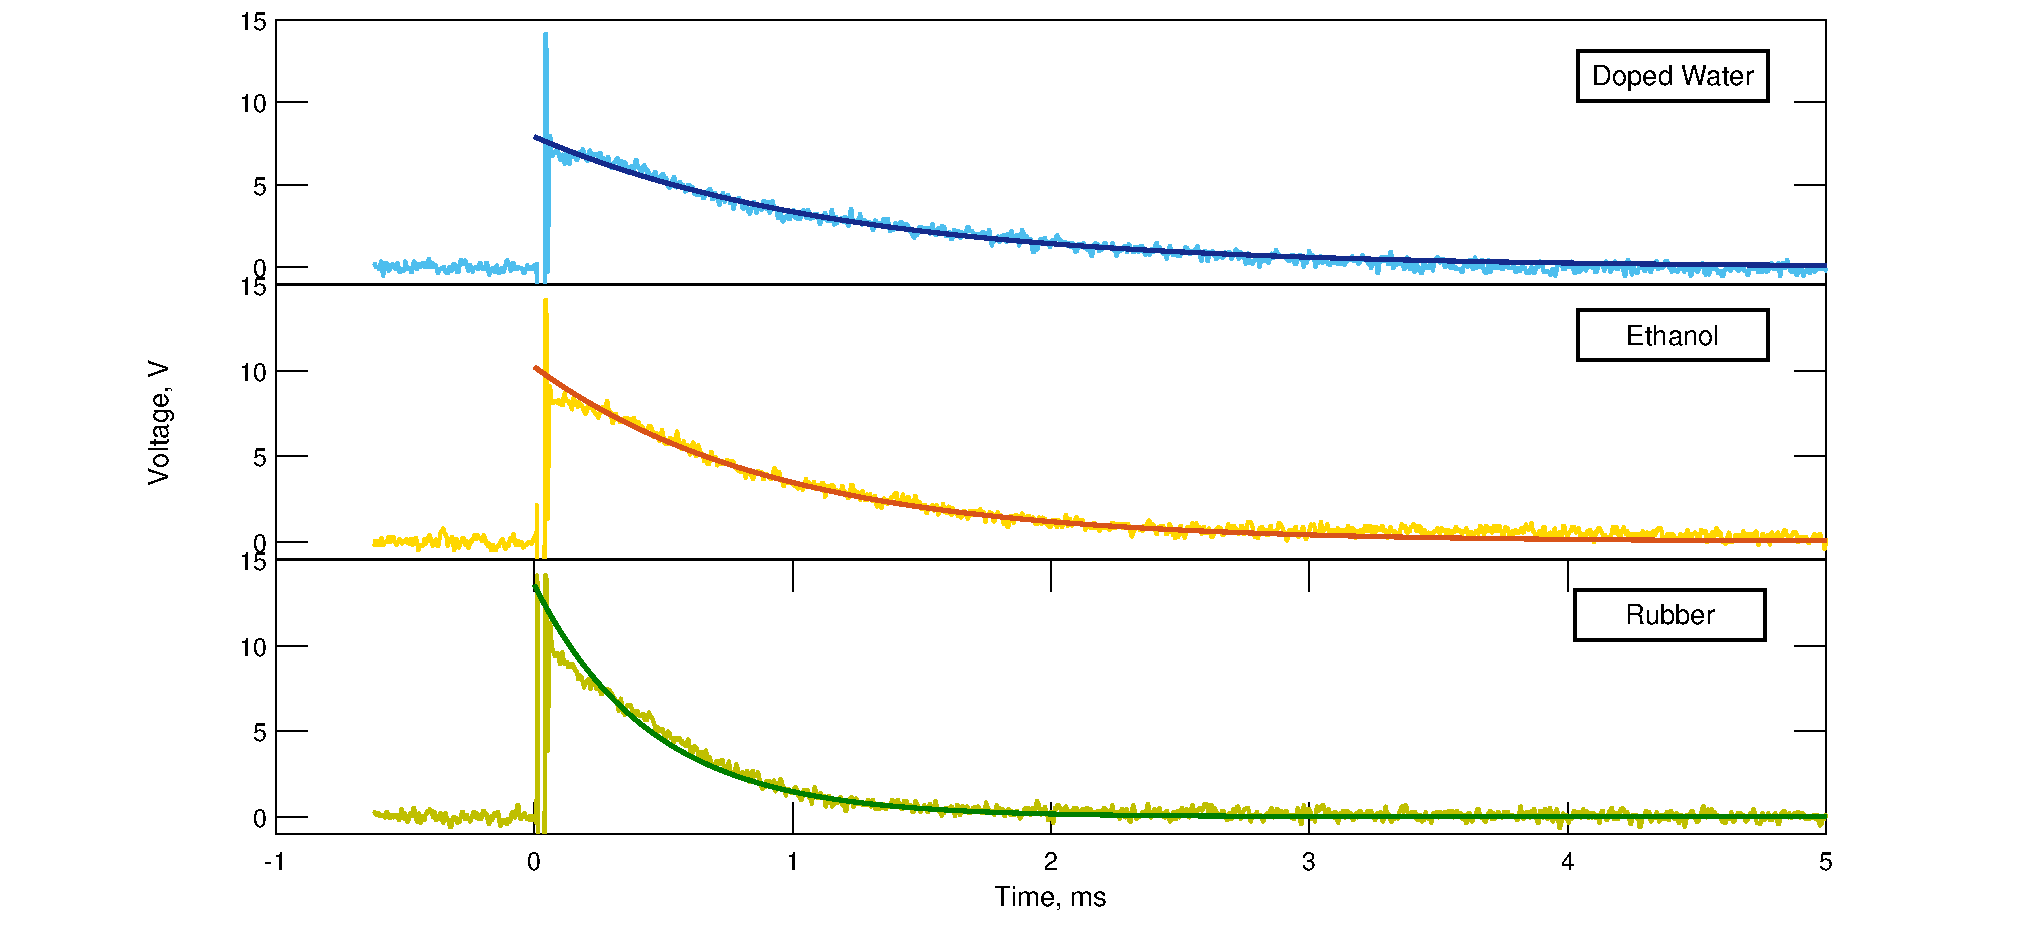
\includegraphics[width=\textwidth]{figures/B2/B2_1.eps}
\caption{FID from a 90 degree pulse for doped water, ethanol, and rubber to determine $T_2^*$.}
\label{fig:B2:T2*_samples}
\end{figure}

The behaviour of each fit matches quite well with the experimental data, following the trend very closely. The $R^2$ values in Table \ref{tab:B2:T2*_values} are based off of the linear fit to the natural logarithm (see Figure \ref{fig:A_B2_logfit} in the Appendix).\\

For each sample, directly following the pulse there is a reduction in the peak value from what the theoretical model predicts. This is likely caused by cross-talk effects between the applied pulse and detector -- which is a systematic instrument error and could be reduced by readjusting the spectrometer settings. It could also be that there may be a better method to remove the detector peak.

\begin{table}[H]
    \centering
    \begin{tabular}{c|c|c|c|c}
    \toprule
    \textbf{Sample} & $T_2^*$ Estimate & $T_2^*$ (ms) & $R^2$ & Percent Difference (\%) \\ \midrule
        Doped Water & $1.4110\pm0.1472$ & $1.169 \pm 0.017$ & $0.9324$  & $18.76$\\
        Ethanol & $1.2270\pm0.1472$ & $0.9239 \pm 0.0085$ & $0.9638$ & $28.18$\\
        Rubber & $0.6415\pm0.1104$ & $0.4495 \pm 0.0073$ & $0.9550$  & $35.20$ \\ \bottomrule
    \end{tabular}
    \caption{Summarized values of $T_2^*$ for the three samples. First column is calculated using th estimation of $M_y=M_0/e$, depicted in Figure \ref{fig:B2:T2*_approx}. The second column is calculated from the fits depicted in Figure \ref{fig:B2:T2*_samples}, with the corresponding $R^2$ goodness-of-fit value.}
    \label{tab:B2:T2*_values}
\end{table}

Comparing the two methods summarized in Table \ref{tab:B2:T2*_values}, we see that the estimated value of $T_2^*$ is always greater than the calculation using a fit. 


%Its possible that this is caused by deconstructive interference from the sharp peak that we see from the instrument? I remember it creates a peak like a damped harmonic oscillator and may have some effect like we see. I'll have to actually look at the scans we took before establishing this for sure.

\subsection{Finding \texorpdfstring{$T_{1}$}{T1} for Water, Ethanol and Rubber Using Saturation Recovery Sequence} \label{B3}

With a 90$\degree$-$\tau$-90$\degree$ pulse sequence, the  magnetic vector regrowth along the $z$-axis is given by equation \ref{eqn:SR},
\begin{align*}
M_z(t) &= M_0(1 - e^{-\tau/T_1} ) \\
\intertext{As the second pulse has been set to have $M_z=M_0/2$, }
\frac{1}{2} &= 1 - e^{-\frac{\tau}{T_{1}}}
\end{align*}
Taking the natural logarithm of both sides and rearranging,
\begin{align*}
T_1 &= \frac{\tau}{\ln 2} \numberthis \label{eqn:B3:T1}
\end{align*}

The time delay between the two pulses, $\tau$, was measured in post-processing by calculating the peaks in of the digital oscilloscope trace data. $\tau$ was set such that, 
\[ M_z\approx M_0/2 \numberthis \label{eqn:B3:M0/2} \]

As the determination of what time delay $\tau$ satisfies Equation \ref{eqn:B3:M0/2} is approximate at best, three data traces were saved and analyzed in post-processing. The three data sets spanned the approximate range of time delays, such that the data sets have peak magnetization of $\lesssim M_0/2$, $\approx M_0/2$ and $\gtrsim M_0/2$. A simple 90$\degree$ FID (as in Section \ref{B1}) was used to calculate a $M_0/2$ in post-processing. A linear slope was fit between the time-delayed peaks of the three approximate data sets (see Figure \ref{fig:B3:example_uncertainty}) and the point on this slope where $M_z = M_0/2$ is our calculated value of $\tau$. $T_1$ is then computed using Equation \ref{eqn:B3:T1}. As there is a large number of error in this measurement caused by uncertainty in the measurement of $M_0$, the peak detection on the saturation recovery peaks, and the linear fit, the uncertainty is taken to encompass the recovery peaks in all three traces. It could be an improvement to take more than three data points to create the line but this is a rough approximation so additional data points were not taken.

%there is large error in the measurement as the recording of $M_0$ was approximated to begin with and measuring half that data is also approximate. So, to determine an uncertainty in $\tau$, three traces were saved in the range of $\tau$ which satisfied Equation \ref{eqn:B3:M0/2} -- one at the lower end, center, and high end. The final value is taken as the mean of the the three $\tau_i$ values, and the uncertainty determined as the minimum value to encompass all three measured values. Mathematically, if the three measure time delays are denoted as $\tau_i$ where $i=1,2,3$, then the final value is,


\begin{figure}[H]
    \centering
    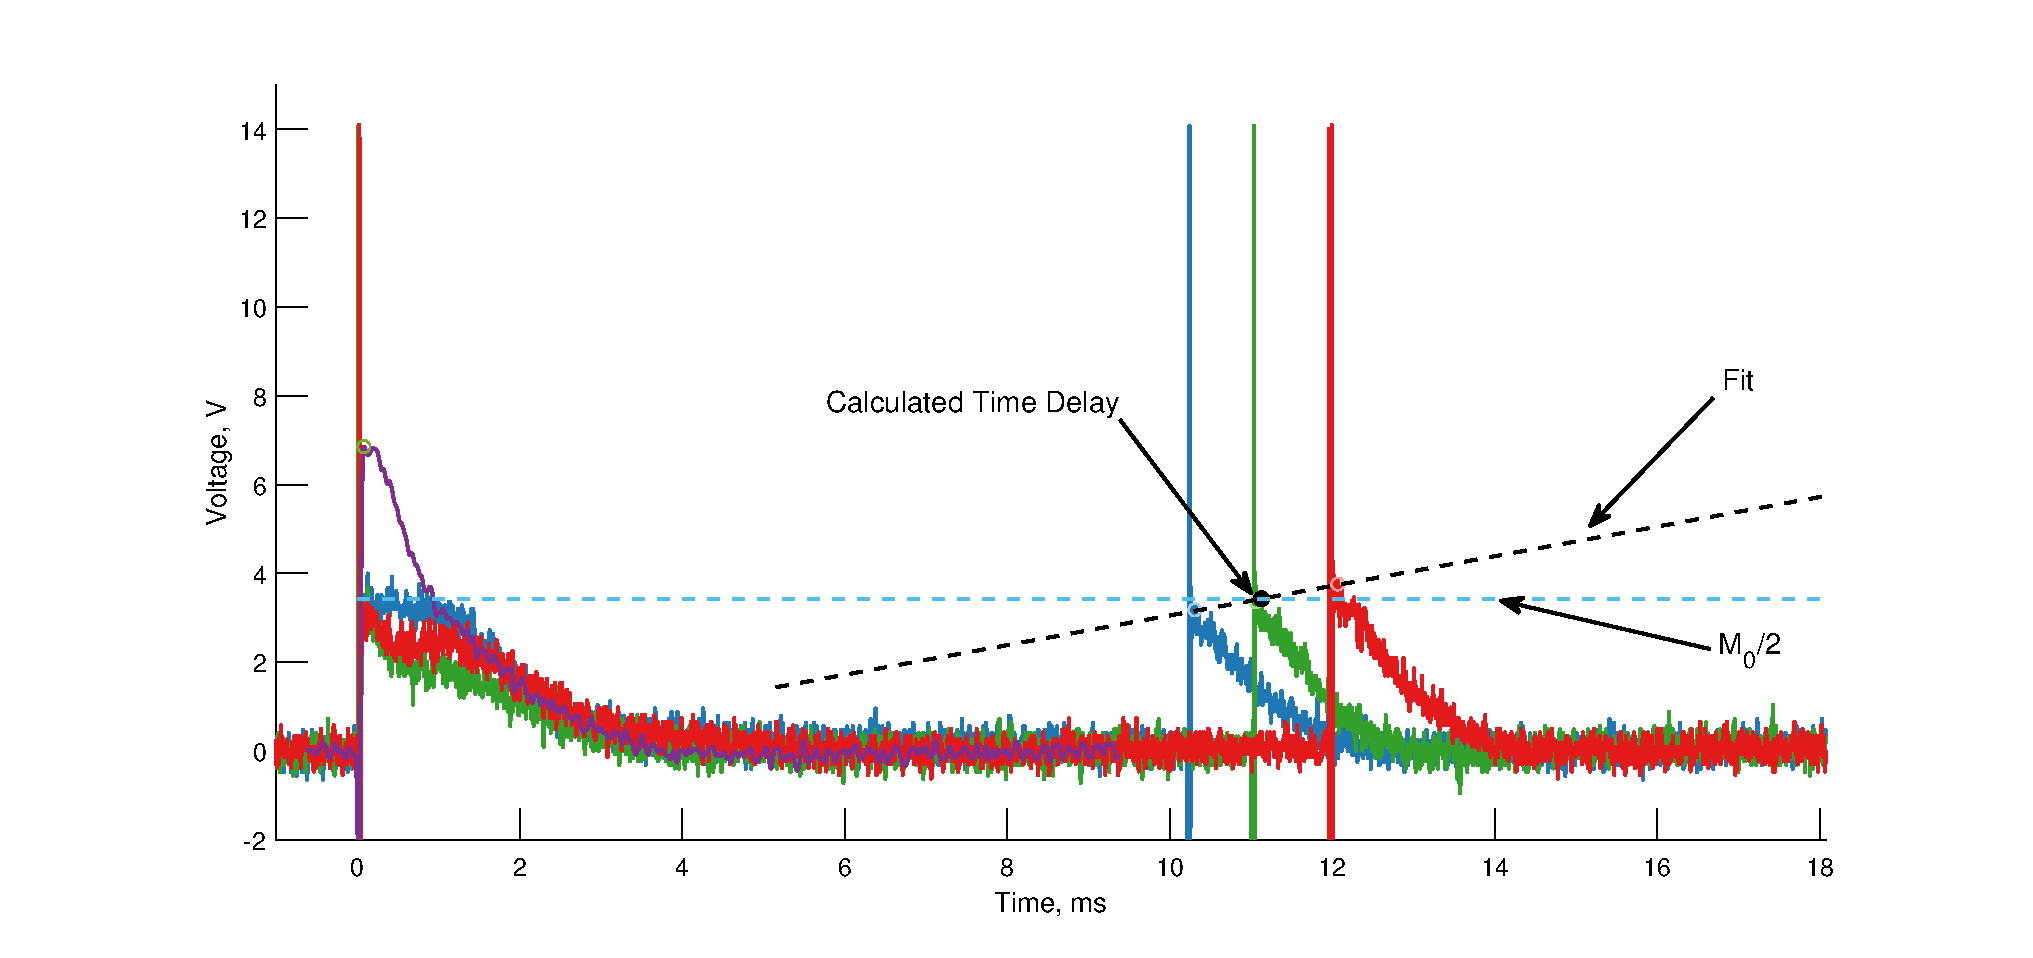
\includegraphics[width=\textwidth]{figures/B3/B3_2.eps}
    \caption{Three doped water saturation recovery traces with $\tau \approx M_0/2$, as well as 90 degree FID (purple trace) to measure $M_0$ with greater precision. Calculated $\tau$ value is shown as black circle and linear fit is dotted black line.}
    \label{fig:B3:example_uncertainty}
\end{figure}

This process was repeated for ethanol and rubber, and the calculated $T_1$ values are tabulated in Table \ref{tab:B3:T1values}.

\begin{table}[H]
    \centering
    \begin{tabular}{c|c}
    \toprule
        \textbf{Sample} & $T_1$ (ms) \\ \midrule
        {Doped Water} & $16.2770  \pm  1.1537$ \\
        {Ethanol} & $1029.1 \pm 80.1$  \\
        {Rubber} & $34.1179 \pm 5.658$ \\ \bottomrule
    \end{tabular}
    \caption{$T_1$ values for three samples, measured using a saturation recovery pulse sequence.}
    \label{tab:B3:T1values}
\end{table}

A second method for estimating $T_1$ can be performed during this experiment. While probing the sample with a 90$\degree$ FID sequence, the signal will decrease rapidly when the repetition rate is approximately equal to $5T_1$. By reducing the pulse repetition rate until no signal is visible, the previous repetition rate is a highly approximated value of $5T_1$. This estimation of $T_1$ is highly imprecise as there is only 5 options for pulse repetition rate with large space between them. Thus, the `resolution' of this method is very low. The calculated time constant would always be greater than its true value, as the last setting \textit{prior} to the signal decrease is used as the estimate. This method was not performed, but could be useful for gaining insight into the order of magnitude and an upper bound for $T_1$.  \\

%To experimentally get the time \textit{t} for which $M(t) = \frac{M_0}{2}$, two 90 degree pulses were applied to the signal and the time was adjusted until the amplitude of the signal equaled $\frac{M_0}{2}$. The time difference between the two pulses is equal to \textit{t} for the $T_1$ calculation above. The two pulses can be identified as the spikes in the graph below:
%\begin{figure}[H]
%\centering
%\label{FIDApprxT1}
%\includegraphics[width=0.6\textwidth]{WaterT1.jpg}
%\caption{FID graph for water illustrating $T_{1}$ approximation.}
%\end{figure}
%From the graph above, we can see that the time difference used to calculate $T_1$ is equal to 0.017244 s. Therefore, using the $T_1$ equation above:
%From this approximation we can see that $T_1$ for water was an order of magnitude larger than $T_{2}^*$.The $T_1$ uncertainty for this method is  hard to approximate 

\subsection{Measuring \texorpdfstring{$T_1$}{T1} for Water, Alcohol and Rubber Using the Inversion Recovery Sequence} \label{B4}

\begin{comment}
\begin{itemize}
\item Write at the beginning of this section what the inversion recovery sequence is and how we are using it to measure $T_1$ \textbf{(5 mins)}
\item It says to use a repetition time at least 5*$T_1$. Why do we do that? How does it impact our data? Discuss here \textbf{(5 min)}
\item Show how you found the initial magnetization data points for one of the samples ****this involves probably shifting the graphs up so that they approach 0****  (show a plot with a labeled data point) \textbf{(10 min)}
\item write up a sample uncertainty calculation for getting one of the values (the uncertainty is the uncertainty associated from reading off the graph + noise), include that calculation in the report. There will be an uncertainty associated with both the time and magnetization values \textbf{(10 mins)}
\item get each value for the initial magnetization and the time for each trial for every sample, record the uncertainties if they differ between different samples because of a difference in scale \textbf{(30 mins)}
\item plot the values obtained for each of the samples, include a graph with error bars (the uncertainties from above), there should be horiziontial and vertical bars because we're approximating both the time and voltage. given units and a title. \textbf{(15 mins)}
\item write up the rearrangement of the $T_1$ equation where you take a the ln and plot the corresponding relationship for each sample \textbf{(30 mins)}. 
\item Use a linear regression (specify which program and function you used) to find $T_1$ for each of the samples. Put in the coefficients with uncertainties that your linear regression outputted. \textbf{(15 mins)}
\item Show a sample calculation for calculating $T_1$ using the equation. Include sample uncertainity calculation. \textbf{(10 mins)}
\item Write up what the zero-crossing method is. \textbf{(5 mins)}.
\item Calculate $T_1$ and its uncertainty for each using the zero-crossing method. Show sample uncertainty calculation. \textbf{(30 mins)}
\item Compare the $T_1$ from inversion to zero crossing using the \% difference for each sample. Show a sample calculation. \textbf{(15 mins)}
\item Talk about why the $T_1$'s are different for each of the samples and the physics. 
\end{itemize}
\end{comment}

An inversion recovery (IR) protocol was performed on the three samples using a 180-$\tau$-90 pulse sequence and all parameters set to maximize the signal. This method is called inversion recovery as the magnetization is initially \textit{inverted} to the negative $z$-direction. As it \textit{recovers} to the positive $z$-direction, the second 90$\degree$ pulse knocks whatever total magnetization is in the $z$ direction to the $xy$-plane -- essentially probing what amount the magnetization has recovered in the time $\tau$.\\

The magnetization at the time-delay of $\tau$ is given by equation \ref{eqn:IR},
\begin{align*}
    M_z(\tau) &= M_0(1-2e^{-\tau/T_1} )\\
    \intertext{Rearranging and taking the natural logarithm of both sides,}
     -\frac{\tau}{T_1} &= \ln \left( \frac{1}{2} -\frac{M_z(\tau)}{2M_0} \right) \numberthis\label{eqn:B4:lnfit}
\end{align*}

Each data trace was zero-shifted and filtered using a Gaussian filter (discussed in Appendix \ref{append:process}), followed by a simple peak detection to determine the time-delay $\tau$ and the peak magnetization $M_z(\tau)$ (see Figure \ref{fig:B4:timetraces}). The initial magnetization, $M_0$, was recorded as the maximum of a single FID for each sample (see, for example, Figure \ref{fig:B1:pulses}). These values were extracted from each experiment and compiled in Figure \ref{fig:B4:expfit}. Using Equation \ref{eqn:B4:lnfit} to fit the data to linear slope we calculate $T_1$ for each sample, which are tabulated in Table \ref{tab:B4:T1vals}. \\

The $T_1$ values for each sample can also be calculated using the zero-crossing (ZC) method. From Equation \ref{eqn:B4:lnfit} with $M_z(t) = 0$,
\begin{align*}
    T_1 &= \frac{\tau}{\ln(2)} \numberthis
\end{align*}

So, using the above equation with a rough estimate of the value for $\tau$ where $M_z(\tau)=0$ we can generate a rough guess of $T_1$.

\begin{figure}[H]
    \centering
    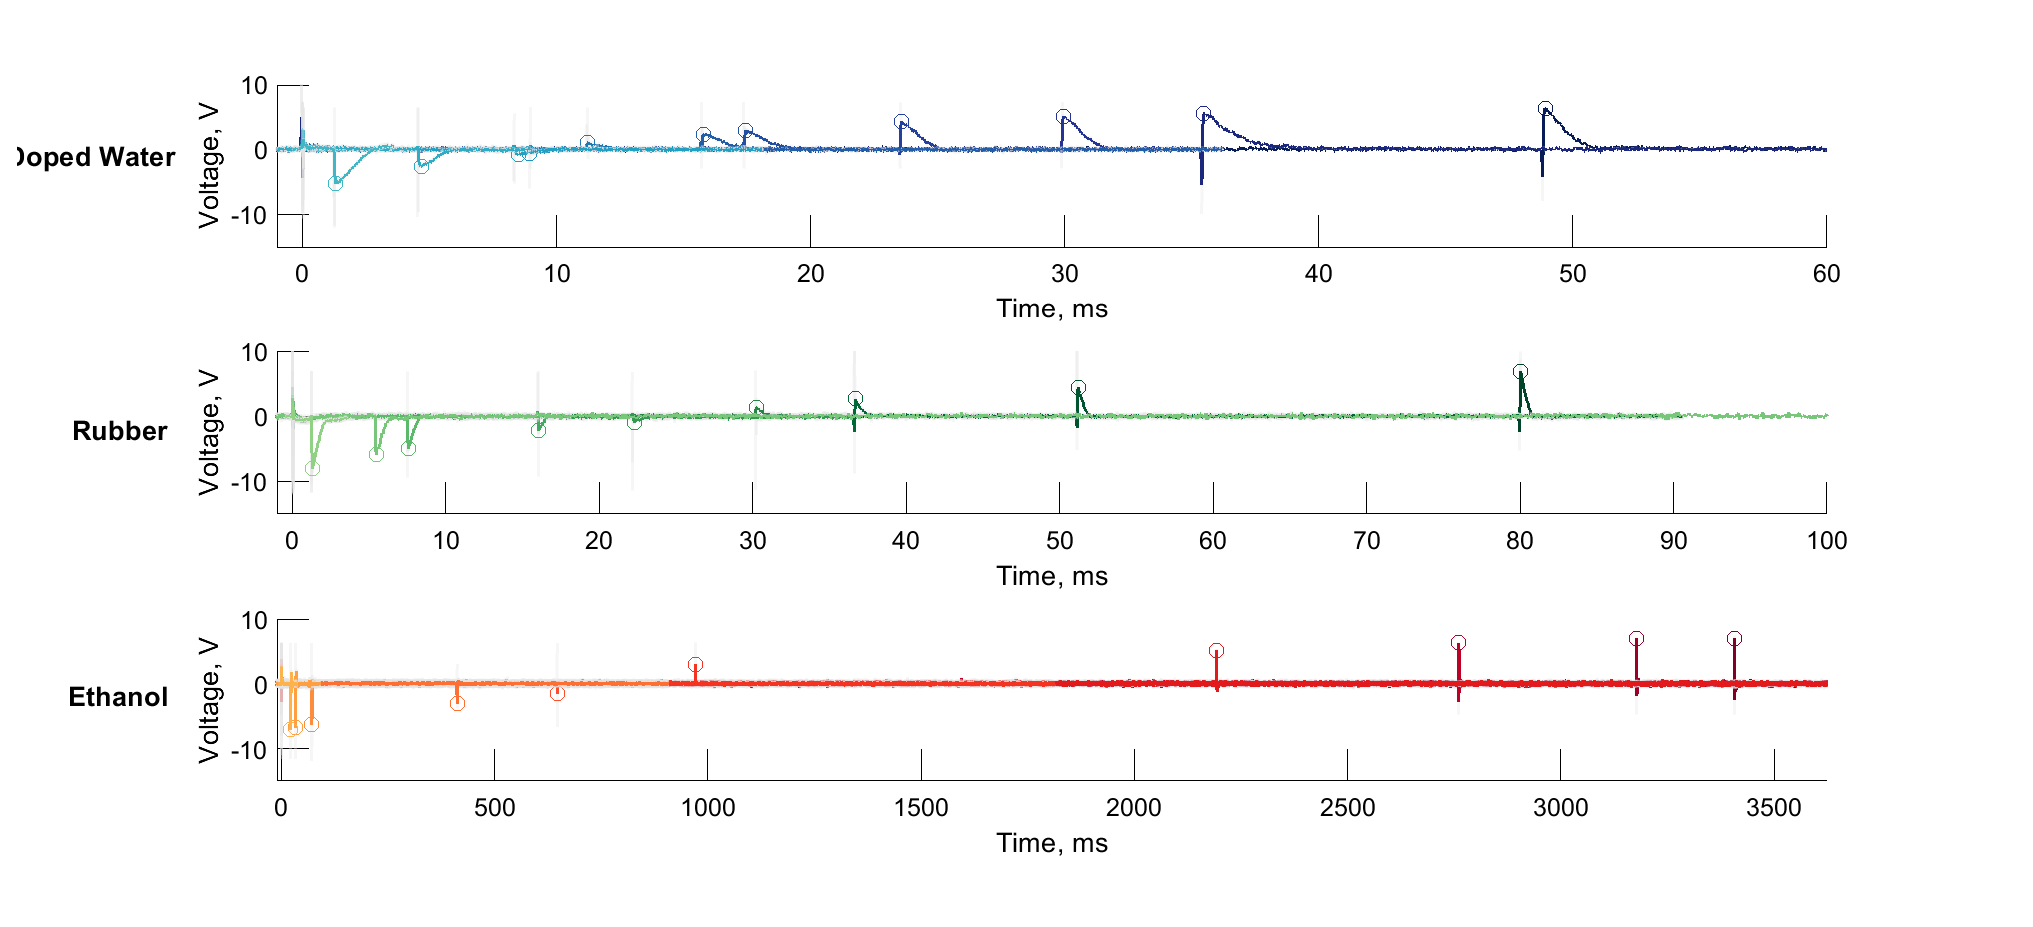
\includegraphics[width=\textwidth]{figures/B4/B4_1.eps}
    \caption{Oscilloscope traces of IR sequence for three samples after zero-shifting and filtering to determine peak magnetization values for each value of $\tau$. Solid lines are the filtered data, light gray lines represent the raw, unfiltered data, and circles represent the computed peak magnetization values at $\tau$.}
    \label{fig:B4:timetraces}
\end{figure}

\begin{figure}[H]
    \centering
    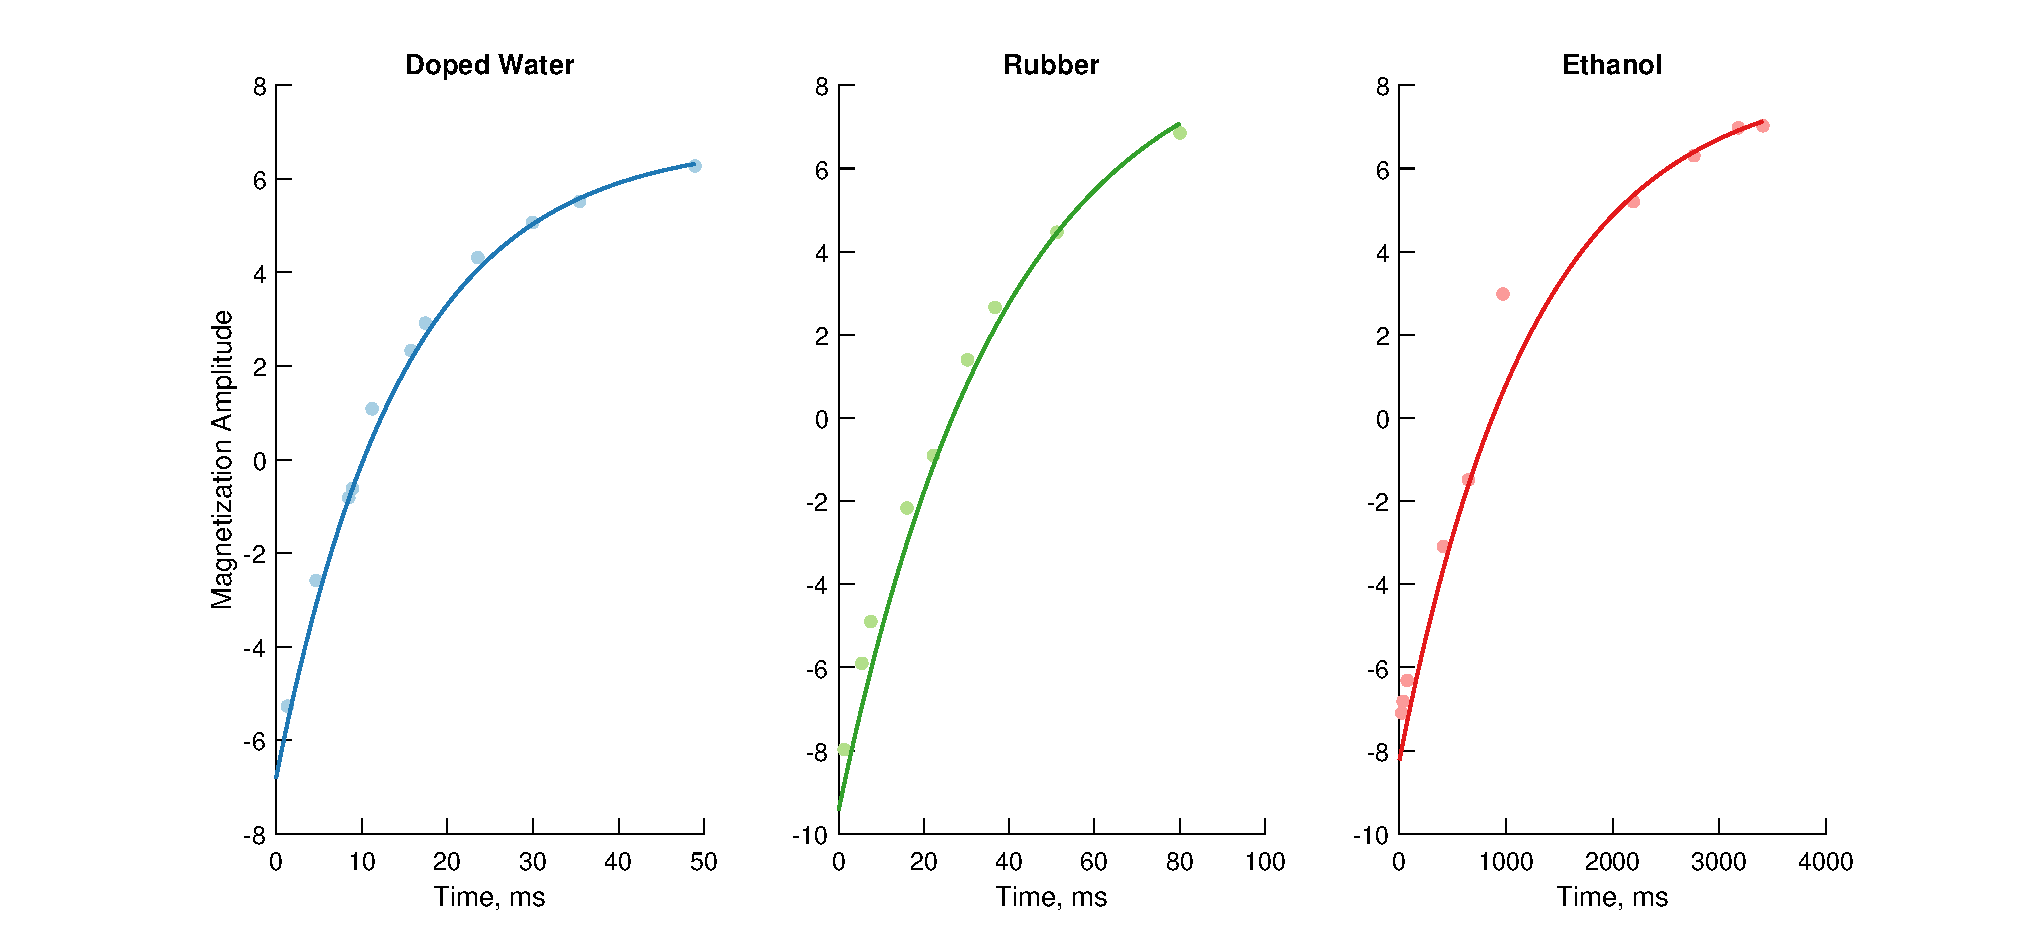
\includegraphics[width=\textwidth]{figures/B4/B4_2.eps}
    \caption{Peak magnetization values at a time-delay of $\tau$ (coloured circles) with the corresponding fit (solid line), calculated from the traces demonstrated in Figure \ref{fig:B4:timetraces} for doped water, ethanol and rubber.}
    \label{fig:B4:expfit}
\end{figure}

\begin{table}[H]
    \centering
    \begin{tabular}{c|c|c|c}
    \toprule
    \textbf{Sample} & IR Method $T_1$ (ms) & ZC Method $T_1$ (ms) & Percent Difference (\%)\\ \midrule
        Doped Water &  $14.74 \pm 0.41$ & $14.0\pm1.2$ & 5.15 \\
        Ethanol &  $1257 \pm 82$ & $1117\pm168$ & 11.79 \\
        Rubber &  $38.48 \pm 2.09$ & $37.2\pm 3.1$ & 3.38 \\ \bottomrule
    \end{tabular}
    \caption{$T_1$ values for three samples calculated using the inversion-recovery (IR) sequence (fit parameters from Figure \ref{fig:B4:expfit}), the zero-crossing (ZC) method, and the percent difference between the two methods.}
    \label{tab:B4:T1vals}
\end{table}

The uncertainty range of the ZC method always encloses the value calculated from the IR value, as the uncertainty in the ZC method is highly inaccurate. However this does not hold true vice versa, as the uncertainty in the IR measurements is much lesser and does not encompass the ZC method values. For ethanol, as the time scales are much longer, it is difficult to generate an accurate estimation of where the zero-crossing point is -- which is reflected in the percent difference from our more accurate IR method. The ZC method is a suitable procedure for estimating the $T_1$ constant, but as it is based off a single point, is not suitable for as a true measurement.\\ 

We may also compare this method to that used in Section \ref{B3}. Comparing the values of $T_1$ using the IR method (Table \ref{tab:B4:T1vals}) and the SR method (Table \ref{tab:B3:T1values}), the percent differences are $9.91\%$ for doped water, $19.94\%$ for ethanol, and $11.84\%$ for rubber. While both the IR and SR methods have limitations and errors, the IR method is more accurate for calculating $T_1$ -- as generating a fit over many data points reduces the propagation of random errors, which does not happen in Section \ref{B3} with the SR method. Thus, $T_1$ values calculated using the IR method, tabulated in Table \ref{tab:B4:T1vals}, are considered as our most realistic time constants. \\

\subsection{Hahn Echo} \label{B5}

\begin{comment}
\begin{itemize}
\item talk about what the hahn echo is and how we're measuring it \textbf{(10 mins)}
\item Show how you found the magnetization data points for one of the samples ****this involves probably shifting the graphs up so that they approach 0****  (show a plot with a labeled data point) \textbf{(10 min)}
\item find the magnetization data points for each of the graphs and uncertainties \textbf{(15 mins)}
\item plot the values obtained for each of the samples, include a graph with error bars (the uncertainties from above), there should be horiziontial and vertical bars because we're approximating both the time and voltage. given units and a title. \textbf{(15 mins)}
\item fit an exp to each plot and say which function and language you're using \textbf{(15 mins)}
\item say the coefficients of the each fit and the uncertainties \textbf{(10 mins)}
\item show a sample calculation for $T_2$ and its uncertainty \textbf{(10 mins)}
\item talk about each of the fits, causes for errors etc. and the physics for why the $T_2$'s may be different \textbf{(15 mins)}
\end{itemize}
\end{comment}




The raw data collected from the spectrometer was zero-shifted and smoothed using a simple Gaussian filtering procedure (see Appendix \ref{append:process}). The peak magnetization of the echo decays as,
\begin{align*}
    M(t) &= M_0 e^{-t/T_2}\\
    \intertext{Similar to previous sections, taking the natural logarithm and rearranging,}
    \ln \left( M(t) \right) &= \frac{-t}{T_2} + \ln(M_0) \numberthis \label{eqn:B5:log}
\end{align*}

Figure \ref{fig:B5:fit/trace} shows each trace with different time-delays and the calculated echo amplitude. These amplitudes are plotted against $t=2\tau$ in Figure \ref{fig:B5:expcurve}, along with the fit -- which was determined using a linear least squares regression of the data, using the form from Equation \ref{eqn:B5:log}. From the fit, the $T_2$ value is the slope of the line, and the uncertainty is the 95\% confidence interval of the least squares algorithm. The $T_2$ values for doped water, ethanol and rubber are summarized in Table \ref{tab:B5:T2vals}.

\begin{figure}[H]
    \centering
    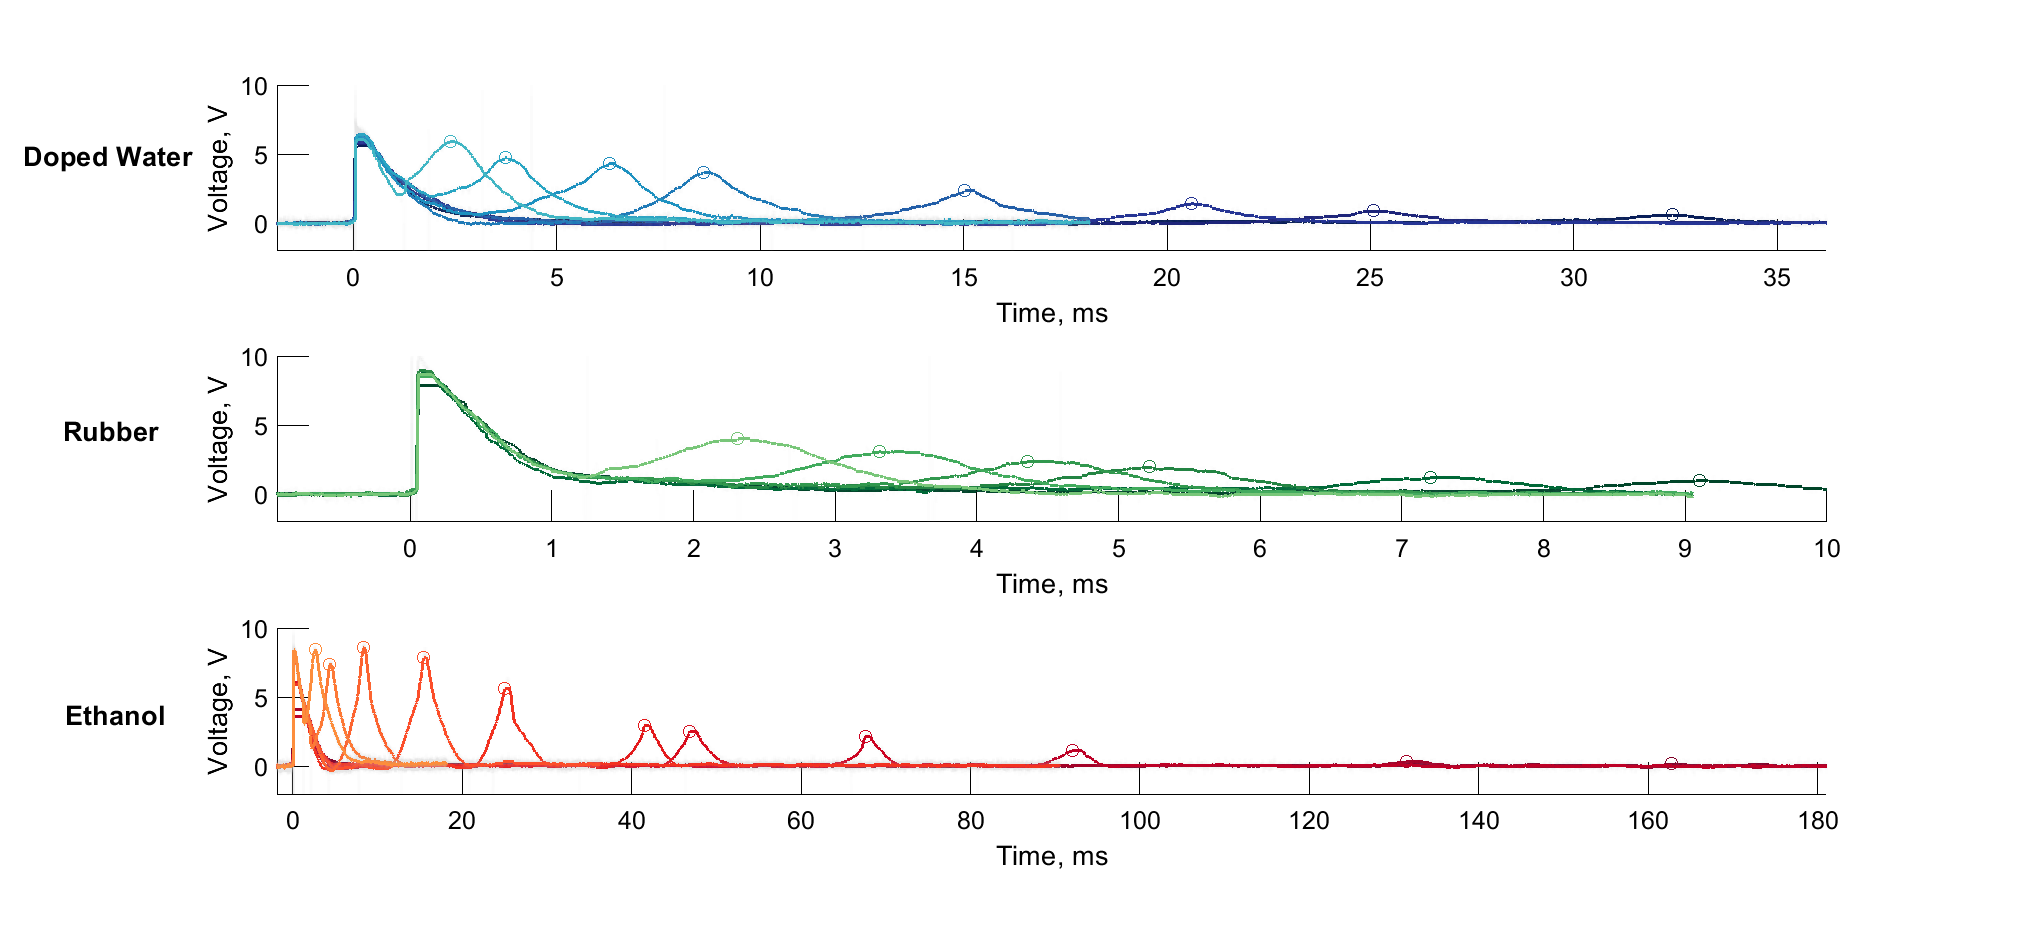
\includegraphics[width=\textwidth]{figures/B5/B5_1.eps}
    \caption{Time traces of Hahn echo experiments for the samples, with multiple traces for time-delay $\tau$ overlaid. The solid lines are the filtered data, light grey is the raw, unfiltered data, and the circle points are the calculated peak magnetization values at $t=2\tau$.}
    \label{fig:B5:fit/trace}
\end{figure}

\begin{figure}[H]
    \centering
    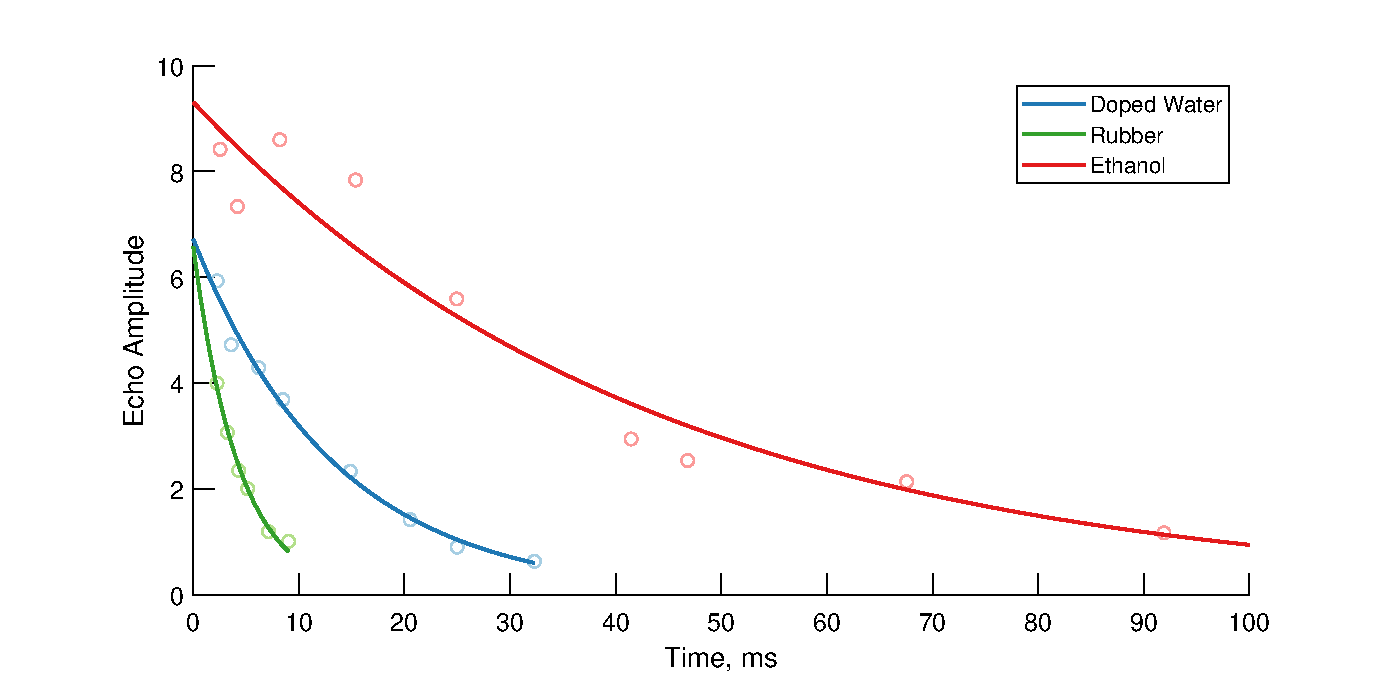
\includegraphics[width=\textwidth]{figures/B5/B5_2.eps}
    \caption{Peak magnetization of three samples, extracted from Figure \ref{fig:B5:fit/trace} to determine $T_2$.}
    \label{fig:B5:expcurve}
\end{figure}

\begin{table}[H]
    \centering
    \begin{tabular}{c|c}
    \toprule
    \textbf{Sample} & $T_2$ (ms) \\ \midrule
        Doped Water &  $13.31 \pm 1.16$ \\
        Ethanol &  $42.21 \pm 3.38$ \\
        Rubber &  $4.80 \pm 1.11$ \\ \bottomrule
    \end{tabular}
    \caption{$T_2$ values for three samples determined using the Hahn echo experiments, calculated from the fit of results from Figure \ref{fig:B5:expcurve}.}
    \label{tab:B5:T2vals}
\end{table}

As expected from Equation \ref{eqn:Hanecho}, 
\[ 1/T^*_2 = 1/T_2 + \gamma \Delta B_o \]
all values of $T_2$ are greater than that of $T_2^*$ (Table \ref{tab:B2:T2*_values}). Using these two terms, it is straightforward to calculate the $\gamma\Delta B_o$ values for each sample. As $\gamma$ is constant for each sample (the gyromagnetic ratio of a proton) then from Table \ref{tab:B5:hom} we can compare the relative field inhomogeneities of each sample. We can see that rubber has greater field inhomogeneities than the liquid sample ethanol by a factor of approximately two. The rubber sample used here, a pencil eraser, likely has manufacturing impurities and spatial differences in density and chemical composition -- compared to a highly pure sample of ethanol. Thus, it is consistent with our knowledge of the samples that the field inhomogeneities of rubber are greater than the other two samples. 
\begin{table}[H]
    \centering
    \begin{tabular}{c|c} \toprule
        \textbf{Sample} & $\gamma \Delta B_o$ (ms$^{-1}$) \\ \midrule
        Doped Water & $0.7876\pm0.0126$ \\
        Ethanol & $1.0816\pm0.0100$ \\
        Rubber & $2.1987\pm0.0362$ \\ \bottomrule
    \end{tabular}
    \caption{Comparison of the field inhomogeneities for each sample, computed from the differences in $T_2$ (Section \ref{B4}, IR method) and $T_2^*$ (Section \ref{B2}).}
    \label{tab:B5:hom}
\end{table}

\subsection{Freezing} \label{B6}

This section of the experiment relied upon freezing our sample of doped water. Our graphs for the FID of ice vs water are shown in Figure \ref{fig:B6:icewater}. We clearly see that frozen water has no visible excitation.

\begin{figure}[H]
    \centering
    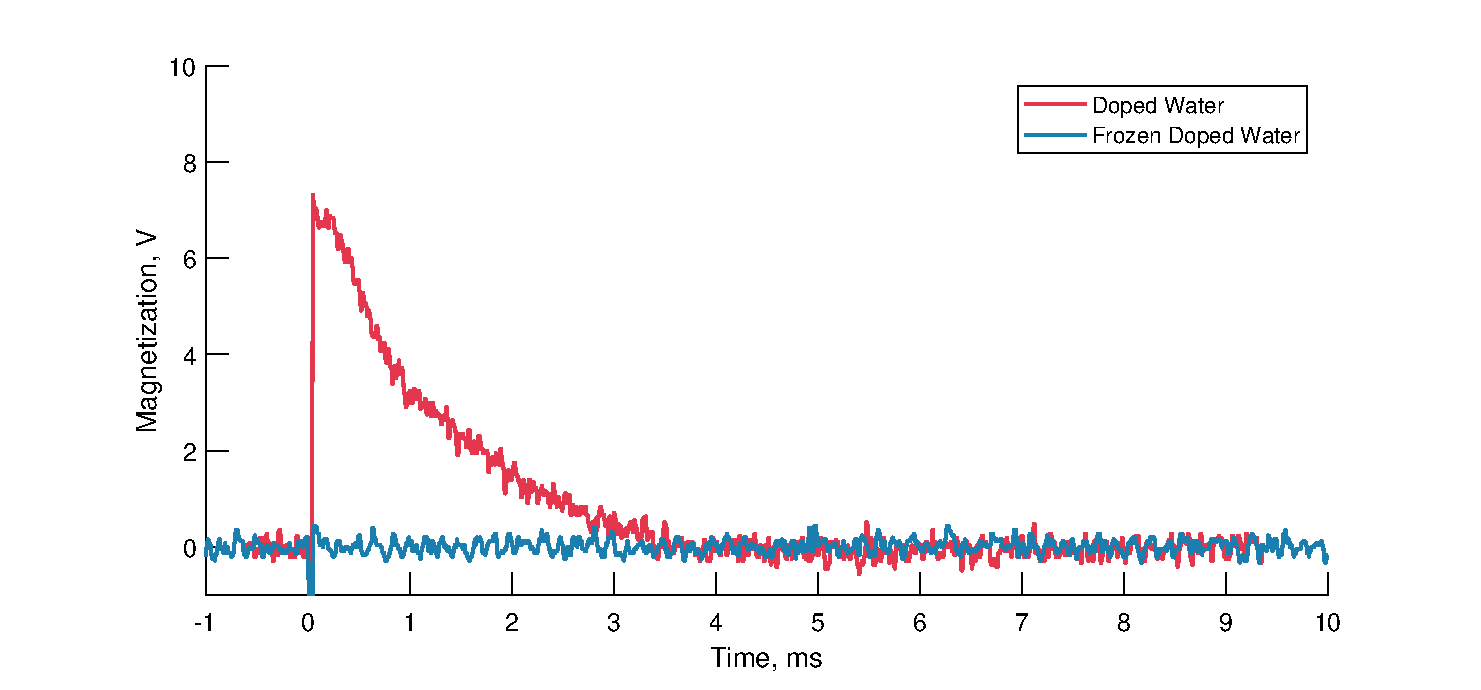
\includegraphics[width=\textwidth]{figures/B6/B6_1.eps}
    \caption{Example FID of doped water at room-temperature (liquid) and frozen (solid).}
    \label{fig:B6:icewater}
\end{figure}

To explain this we note that in our derivation of $\vec{M}$, the magnetization vector, we assumed that each atom could rotate independently, which is true in a liquid, but is an untrue assumption when working with a solid. In a solid, orientation dependant effects are observed. Some examples of these effects are non-averaged dipolar interactions and chemical shift anistropy interactions. These non-averaged effects lead to the case where resonances are very broad. 

To compare these liquid vs solid resonances it is typical to compare line width which is known to be $<$ 1 Hz in liquid water while the resonances in ice is broadened up to \textapprox $10^5$ Hz. \cite{bakhmutov2015nmr} This means that a radio frequency signal to affect the magnetization would have to be broadband. To achieve a good signal the frequency needed to excite are generally around 50-100 kHz. \cite{bakhmutov2015nmr}. \\

In this experiment we excite with a single frequency, so due to this broad peak we are unable to resonate with a large amount of the atoms and hence we cannot change their orientation with the Rabi pulses, leading to a lack of signal.\\

Also, the spin lattice relaxation time ($T_1$) requires interactions with the external world, as it is due to thermal effects such as molecular rotation, diffusion, or lattice vibration \cite{fukushima1981experimental}, hence it can be very weak in the absence of molecular motion, as is in the case of low temperature crystalline structures such as frozen water. This means that the $T_1$ times of ice water are much larger than that of liquid waters. The ice water relaxation time has been measured to be 39.40s \cite{le2000study}. To gain a FID signal enough time must elapse between the successive pulses in order for the magnetization to build up along the $z$-axis so that the signal is large. Hence our repeat times which were 0.3s were such that the signal could not have been seen. 



%As we can see from Figure \ref{fig:B6:icewater}, there is no signal (using all the same experimental parameters) when the water is frozen.


\subsection{Comparison of Rubber and Ethanol}

Here we briefly discuss some of the results and how they apply to the three samples. Note that the doped water is essentially a calibration sample as it has been modified to increase its signal. Hence we will investigate the differences between ethanol and rubber.\\

In analyzing these results, we can conclude that the time constants for ethanol are an order of magnitude larger than that of a rubber. The typical designation of ``rubber'' commonly refer to a class of polymers known as elastomers (although this is not completely accurate in specific cases \cite{polydict}). These elastomers have high molecular mobility and narrow NMR lines due to their weak intermolecular forces between their polymer chains,  \cite{NMRpoly}. These characteristics make them ideal for pulse NMR spectroscopy as the high molecular mobility has been linked to lower $T_1$ and $T_2$ times, which has been verified in references \cite{polyT1, polyT}. This lowering of $T_1$ and $T_2$ based off of molecular mobility is due to the fact that interactions in general increase with an increase of molecular mobility. These interactions can be molecular collisions, which affect $T_1$ or higher fluctuations in local fields which affect $T_2$.\\

However in comparison the dominant intermolecular force present in ethanol is hydrogen bonding, which is a strong force, which directly leads to a decrease of molecular mobility and hence an increase in both $T_1$ and $T_2$.\\